% !Mode:: "TeX:UTF-8"
% !TEX program  = xelatex
\documentclass[a4paper]{article}
\usepackage{amsmath}
\usepackage{amssymb}
\usepackage{ctex}
\usepackage{graphicx}
%\usepackage{braket}
\usepackage[european]{circuitikz}
\usepackage{multirow}
\usepackage{geometry}
\geometry{left=2.5cm,right=2.5cm,bottom=2.5cm,top=2.5cm}
\title{物理化学实验17:振荡反应}
\author{薛明怡\quad 151250177\quad 化学化工学院}
\date{}
%\date{2019年2月29日}
\begin{document}
\maketitle
\bibliographystyle{unsrt}
\section{实验目的}
\begin{enumerate}
\item 了解Belousov-Zhabotinsli反应的基本原理.
\item 初步理解自然界中普遍存在的非平衡非线性问题.
\end{enumerate}
\section{实验原理}
\subsection{自催化反应}
在给定条件下的反应体系, 反应开始后逐渐形成并积累了某种产物或中间体, 这些产物具有催化功能, 
使反应经过一段诱导期后出现大大加速的现象, 这种作用称为自(动)催化作用. 其特征之一是存在着初始的诱导期. 
大多数自动氧化过程都存在自催化作用. 油脂腐败, 橡胶变质以及塑料制品的老化均属于包含链反应的自动氧化过程, 
反应开始进行很慢, 但都被其所产生的自由基所加速.
\subsection{化学振荡}
有些自催化反应有可能使反应体系中某些物质的浓度随时间(或空间)发生周期性的变化, 
即发生化学振荡, 而化学振荡反应的必要条件之一是该反应必须是自催化反应. 化学振荡现象的发生必须满足如下几个条件:
\begin{enumerate}
    \item 反应必须是敞开体系且远离平衡态, 即$\Delta_{r} G_{m}$为较负的值.
    \item 反应历程中应包含自催化的步骤.
    \item 体系中必须能有两个准定态存在.
\end{enumerate}
\subsubsection{反应机理}
\subsection{}
\section{仪器与药品}
\begin{enumerate}
    \item \textbf{仪器}\\
    \begin{enumerate}
        \item $100$mL 烧杯$1$只
    \end{enumerate}
    \item \textbf{药品}\\
    \begin{enumerate}
        \item 丙二酸(A.R)
        \item 溴酸钾(A.R)
    \end{enumerate}
\end{enumerate}
\section{实验步骤}
\begin{enumerate}
\item \textbf{连接电路}\\
\begin{enumerate}
\item 用多用电表判断实验箱上的三极管的好坏。由于三极管已焊在实验电路板上,无法用多用电表的$h_{EF}$档测量。改用多用表测量二极管档测量。对NPN三极管,用正表笔接基极,用负表笔分别接射极和集电极,多用表应显示PN结导通;再用负表笔接基极,用正表笔分别接射极和集电极,多用表应显示PN结截止。这说明该三极管是好的。用多用表判断实验箱上电解电容的好坏。对于10$\mu F$电解电容,可选择200$k\Omega$电阻测量档,用多用表的负极接电解电容的负极,用多用表的正极接电解电容的正极,多用表的电阻示数将不断增加,知道超出示数范围。这说明该电解电容是好的。
\item 按图(\ref{fig1})连接电路。
\begin{figure}[!h]
\begin{center}
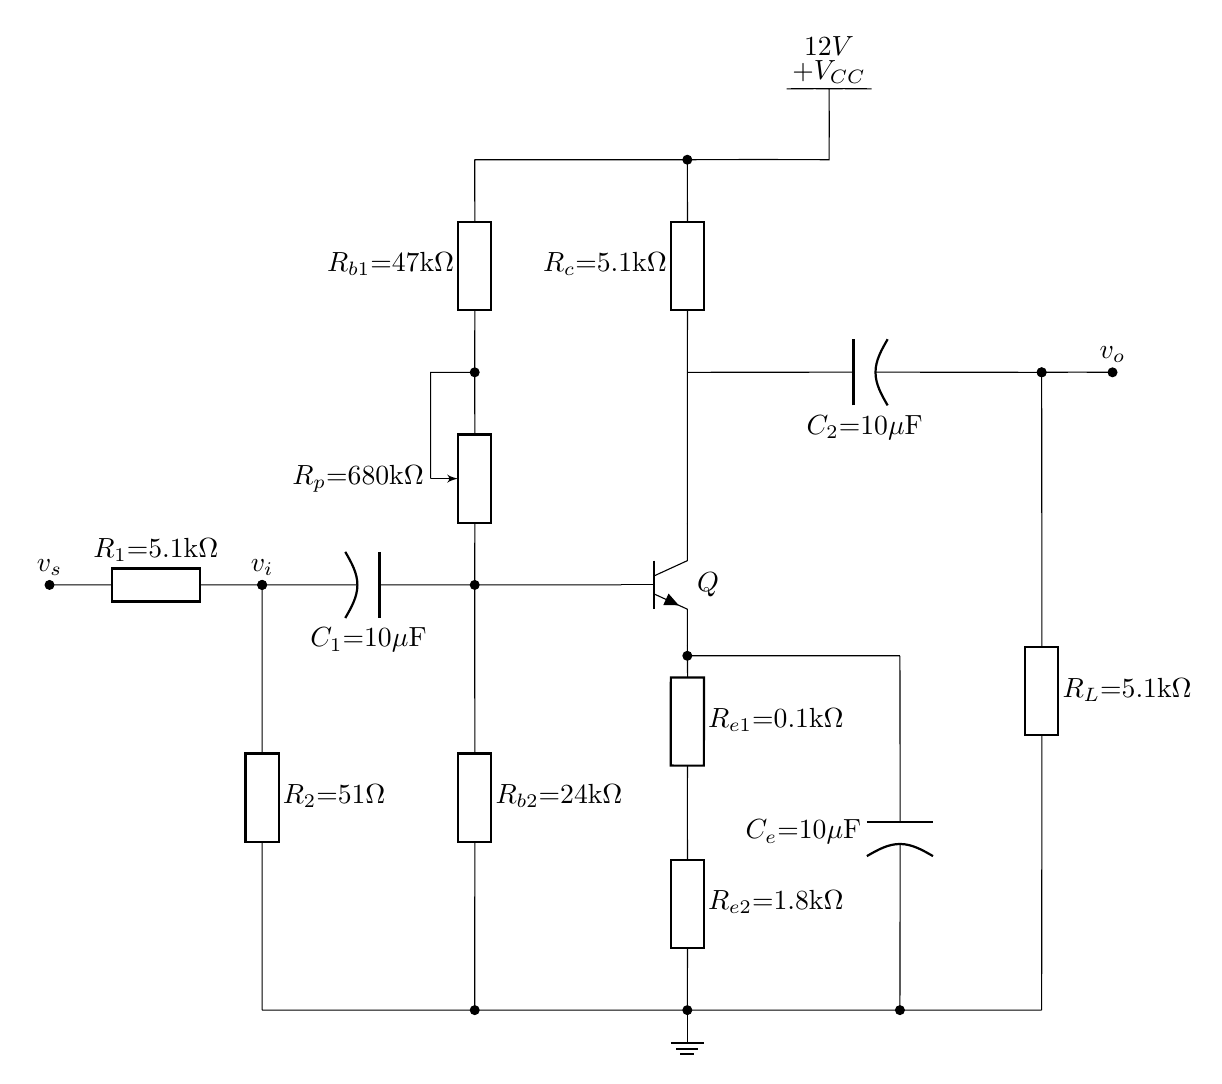
\begin{tikzpicture}[scale=1.8]
    \draw[color=black]
    (0,3) to [R, l = $R_1{=}5.1\text{k}\Omega$, *-*] (1.5,3)
    (1.5,3) to [R, l = $R_2{=}51\Omega$] (1.5,0)
    (1.5,3) to [pC, l_ = $C_1{=}10\mu\text{F}$, *-*] (3,3)
    (3,3) to [R, l = $R_{b2}{=}24\text{k}\Omega$] (3,0)
    (3,3) to [pR, l = $R_p{=}680\text{k}\Omega$, n = PR, -*] (3,4.5)
        to [R, l = $R_{b1}{=}47\text{k}\Omega$] (3,6)
    (3,4.5) -| (PR.wiper)
    (4.5,3) node[npn](NPN){}
    (3,3) to [-] (NPN.B)
    (NPN.E) to [R, l = $R_{e1}{=}0.1\text{k}\Omega$] (4.5, 1.5) to [R, l = $R_{e2}{=}1.8\text{k}\Omega$] (4.5,0)
    (NPN.C) to [-] (4.5,4.5) to [R, l = $R_c{=}5.1\text{k}\Omega$] (4.5,6) to [-] (3,6)
    (4.5,6) to [short, *-] (5.5,6)
    to [short] (5.5,6.5) to [short] (5.2,6.5) to [short] (5.8,6.5) to [short] (5.5,6.5)
    (5.5, 6.8) node{$12V$}
    (5.5, 6.62) node{$+V_{CC}$}
    (7,4.5) to [pC, *-, l = $C_2{=}10\mu\text{F}$] (4.5,4.5)
    (7,4.5) to [short, *-*] (7.5,4.5)
    (7,4.5) to [R, l = $R_L{=}5.1\text{k}\Omega$] (7,0)
    (4.5,2.5) to [short, *-] (6,2.5)
    (6,0) to [pC, l = $C_e{=}10\mu\text{F}$] (6,2.5)
    (1.5,0) to [short, -*] (3,0) to [short, -*] (4.5,0) to [short, -*] (6,0) to [-] (7,0)
    (4.5,0) node[ground](GND){}
	
    {[anchor = south] (0,3) node{$v_s$}}
    {[anchor = south] (1.5,3) node{$v_i$}}
    {[anchor = south] (7.5,4.5) node{$v_o$}}
    {[anchor = west] (4.5,3) node{$Q$}}
;
\end{tikzpicture}
\end{center}
\caption{共射放大电路}\label{fig1}
\end{figure}
\item 接通实验箱交流电源,用多用表测量直流12V电源电压是否正常。若正常,则将12V电源接至图(\ref{fig1})的$V_{CC}$处。
\item 测量电阻$R_c$的阻值。将$v_i$端接地。改变$R_P$(有22$k\Omega$,100$k\Omega$,680$k\Omega$三个可变电阻可选择),测量集电极电压$V_c$,求$I_c = \cfrac{V_{CC}-V_{c}}{R_c}$分别为0.5mA,1mA,1.5mA时三极管的$\beta$值。建议使用以下方法:
\begin{equation}
I_b + \frac{V_b}{R_{b2}} = \frac{V_{CC} - V_b}{R_b}, R_b = R_{b1} + R_P, \beta = \frac{I_c}{I_b}
\end{equation}
\end{enumerate}
请注意,电路断电、电阻从电路中开路后才你用多用表测量电阻值。本实验用测电阻、电压值来计算电流值,而不是直接测量电流,是因为本实验电路的电流较小,测量电流的测量误差较测量电压、电阻的误差大。同时还因为测量电流是多用表的内阻较小,使用不当很可能损坏多用表。

\item \textbf{调整静态}\\
电压放大器的主要任务是失真尽可能小地放大电压信号。为了使输出电压失真尽可能小,一般地说,静态工作点Q应选择在输出特性曲线上交流负载线的中点。若工作点选的太高,放大器在加入交流信号后容易引起失真;若选的太低,容易引起截止失真。对于小信号放大器来说,若输出交流信号幅度较小,电压放大器的非线性失真将不是主要问题,因此Q点不一定要选在交流负载线的中点,而可根据其他要求来选择。例如,希望放大器耗电省、噪声低,或输入阻抗高,Q点可选的低一些。\\
将$v_i$端接地,调整$R_P$,使$V_c = 6V$,测量计算并填表,绘制直流负载线,估算静态工作点和放大电路的动态范围;分析发射机直流偏置电阻对放大器动态范围的影响。
\item \textbf{动态特性分析}\\
保持上述静态不变,做以下动态分析。\\
在本实验电路中,在交流信号输入端有一个由$R_1$,$R_2$组成的1/101的分压器。这是因为,信号源是有源仪器,其输出的信噪比随输出信号的减小而降低。所以输出信号电压幅值有下限。例如,目前使用的Agilent 33210A数字式信号源输出正弦电压的最小幅值为50mV。若直接将其作为输入,本实验用的放大器将严重限幅。电阻是无源器件,且阻值较小,而分压器造成的噪声甚少。所以用电阻分压器的达到信噪比较小的小信号。\\
若要对放大倍数做精确测量,也常用电阻作为输入分压器。具体的做法和原因可叙述如下:若要求放大器的放大倍数的$A_V$,用电阻做1/$A_V$的分压器,信号源的输出电压可为几百mV,调整放大器的参数,使输出电压等于输入电压,这样对输入、输出测量的一起在测量过程中就不用换挡。放大倍数本来就是输出/输入的相对关系。虽然一起测量示数往往有绝对误差,用同一档测量两个量,使其相等,这就避免了仪器测量示数具有的绝对误差。这种测量的误差仅仅包含对两个分压电阻测量的误差,通常很小。若直接用小信号做输入,则测量输入、输出将使用不同的档位,即使用了仪器中的不同的电路,而仪器中的不同电路的测量精度是有差别的,由此而来的误差通常比上述用电阻分压器的要大。
\begin{enumerate}
\item 取输入信号$v_i$的频率为10kHz,有效值为3mV,\textbf{观察}$v_s$和$v_o$的波形,比较两者的相位。
\item 保持信号频率不变,不接负载 $R_L$,用交流毫伏表测量电压,填表,观察$v_o$不严重失真时的最大输入值$v_i$,并填表。
\item 保持信号$v_i$的频率f = 10kHz,有效值3mV不变,接入负载$R_L$,测量并填写表(\ref{table4})。在绘制直流负载线的同一张图上绘制交流负载线,分析负载对放大器动态范围的影响。
\item 不接负载,测量绘制放大器的\textbf{空载幅频特性曲线}。\\
请注意,幅频特性曲线的横坐标是常用对数刻度,建议分配特权限的纵坐标使用20lg$|A_V/A_{Vo}|$dB为刻度。当然也可以适应其他的纵坐标刻度,例如20lg$|A_V|$dB。但不应该适应线性刻度坐标。\\

注:测量时要注意交流毫伏表的测量带宽限制,若频率超过其频宽,应采用示波器进行测量。

\item 利用数字式示波器测量放大器的\textbf{非线性谐波失真}。取输入信号f=10kHz,$R_L = 5.1k\Omega$。\\
对输入$v_i$做傅里叶变换,记
\begin{eqnarray}
d_{i2} &=& \frac{\text{二次谐波谱线幅值}}{\text{基波谱线幅值}}\times 100\%\\
d_{i3} &=& \frac{\text{二次谐波谱线幅值}}{\text{基波谱线幅值}}\times 100\%
\end{eqnarray}
以$d_{i2}$为例说明具体的测量计算方法。数字示波器给出的谱线幅值是对数幅值,其参考值为1$V_{rms}$。示波器屏幕上显示的信号的谱线是其在示波器时域屏幕上波形的傅里叶变换,计及了示波器输入放大器的放大倍数。输入信号的谱线的数值可有游标读出。记基波谱线幅值为$L_1$dB,二次谐波谱线幅值为$L_2$dB,则
\begin{equation}
d_{i2} = 10^{\frac{L_2-L_1}{20}}\times 100\%
\end{equation}
对输出做傅里叶变换,记
\begin{eqnarray}
d_{o2} &=& \frac{\text{二次谐波谱线幅值}}{\text{基波谱线幅值}}\times 100\%\\
d_{o3} &=& \frac{\text{二次谐波谱线幅值}}{\text{基波谱线幅值}}\times 100\%
\end{eqnarray}
放大器的二次谐波失真$d_2$,三次谐波失真$d_3$为
\begin{equation}
d_2 = d_{o2}-d_{i2}, d_3 = d_{o3}-d_{i3}
\end{equation}

\end{enumerate}
\item 测量放大器的\textbf{输入输出电阻}
\begin{enumerate}
\item 测量放大器的输入电阻\\
将图(\ref{fig1})中的$R_2$开路后,放大电路输入端等效电路如图(\ref{fig2}),由图可计算出$r_i$。应调整输入电压,使放大器输出失真尽可能小,因为希望测到的输入电阻是放大器微变等效电路的输入电阻,该电阻是线性电阻。建议将输出端接负载,以减小输出电压。
\begin{figure}[!h]
\begin{minipage}[!h]{0.48\textwidth}
\begin{center}
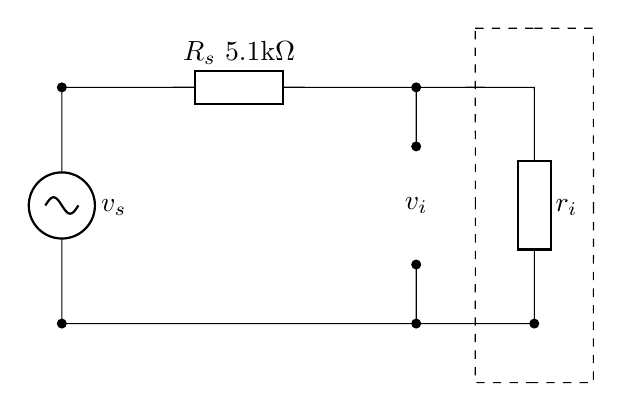
\begin{tikzpicture}[scale=1.5]
    \draw[color=black]
    (0,0) to [sV, l_ = $v_s$, *-*] (0,2)
    (0,2) to [R, l^=$R_s\text{ 5.1k}\Omega$] (3,2)
    to [short, *-*] (3,1.5)
    to [short] (3,2)
    to [short] (4,2)
    to [R,l=$r_i$] (4,0)
    to [short, *-*] (3,0)
    to [short,-*] (3,0.5)
    to [short] (3,0)
    to [short] (0,0)
;
   \draw[dashed]
   (3.5,2.5) to [short] (4.5,2.5)
   to [short] (4.5,-0.5)
   to [short] (3.5,-0.5)
   to [short] (3.5,2.5)
   {(3,1) node{$v_i$}}
;
\end{tikzpicture}
\end{center}
\caption{输入等效电路}\label{fig2}
\end{minipage}
\begin{minipage}[!h]{0.48\textwidth}
\begin{center}
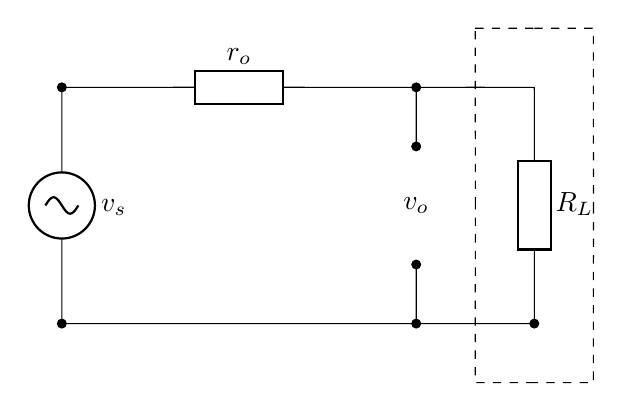
\begin{tikzpicture}[scale=1.5]
    \draw[color=black]
    (0,0) to [sV, l_ = $v_s$, *-*] (0,2)
    (0,2) to [R, l^=$r_o$] (3,2)
    to [short, *-*] (3,1.5)
    to [short] (3,2)
    to [short] (4,2)
    to [R,l=$R_L$] (4,0)
    to [short, *-*] (3,0)
    to [short,-*] (3,0.5)
    to [short] (3,0)
    to [short] (0,0)
;
   \draw[dashed]
   (3.5,2.5) to [short] (4.5,2.5)
   to [short] (4.5,-0.5)
   to [short] (3.5,-0.5)
   to [short] (3.5,2.5)
   
   {(3,1) node{$v_o$}}
;
\end{tikzpicture}
\end{center}
\caption{输出等效电路}\label{fig3}
\end{minipage}
\end{figure}
\begin{equation}
r_i = \frac{R_s}{(V_s/V_i) - 1}
\end{equation}
\item 测量放大器的输出电阻\\
放大电路输出端等效电路如图(\ref{fig3}),此时应将输入端的$R_1,R_2$回复为分压电路,$V_i$为3mV,由图可计算出$r_o$。
\begin{equation}
r_o = \left(\frac{V_{oR_L\to\infty}}{V_{oR_1=5.1k\Omega}}-1\right)
\end{equation}
将输入输出填入表(\ref{table8})。
\end{enumerate}
\end{enumerate}

\section{实验数据}
\begin{enumerate}
\item 静态工作点\\
静态工作点数据如表(\ref{table1}).
\begin{table}[!h]
\centering
\caption{调整静态}
\label{table1}
\begin{tabular}{c|c|c|c|c|c}
\hline
\multicolumn{3}{c|}{测量值}             & \multicolumn{3}{c}{测量计算值}         \\ \hline
$R_b(k\Omega)$ & $V_b(V)$ & $V_e(V)$ & $I_b(\mu A)$ & $I_c(mA)$ & $\beta$ \\ \hline
73.711                  & 2.8659     & 2.2268     & 4.505             & 1.1765       & 261.15        \\ \hline
\end{tabular}
\end{table}
\item 动态分析\\
首先调整输入的函数产生器信号$v_s$使$v_i$为3mV。此时$v_s = 309 mV_{rms}$, $v_i = 3.009 mV$。
观察示波器的输入输出波形如图(\ref{wf})所示,因此相位差为$\pi$。
\begin{figure}[!h]
\centering
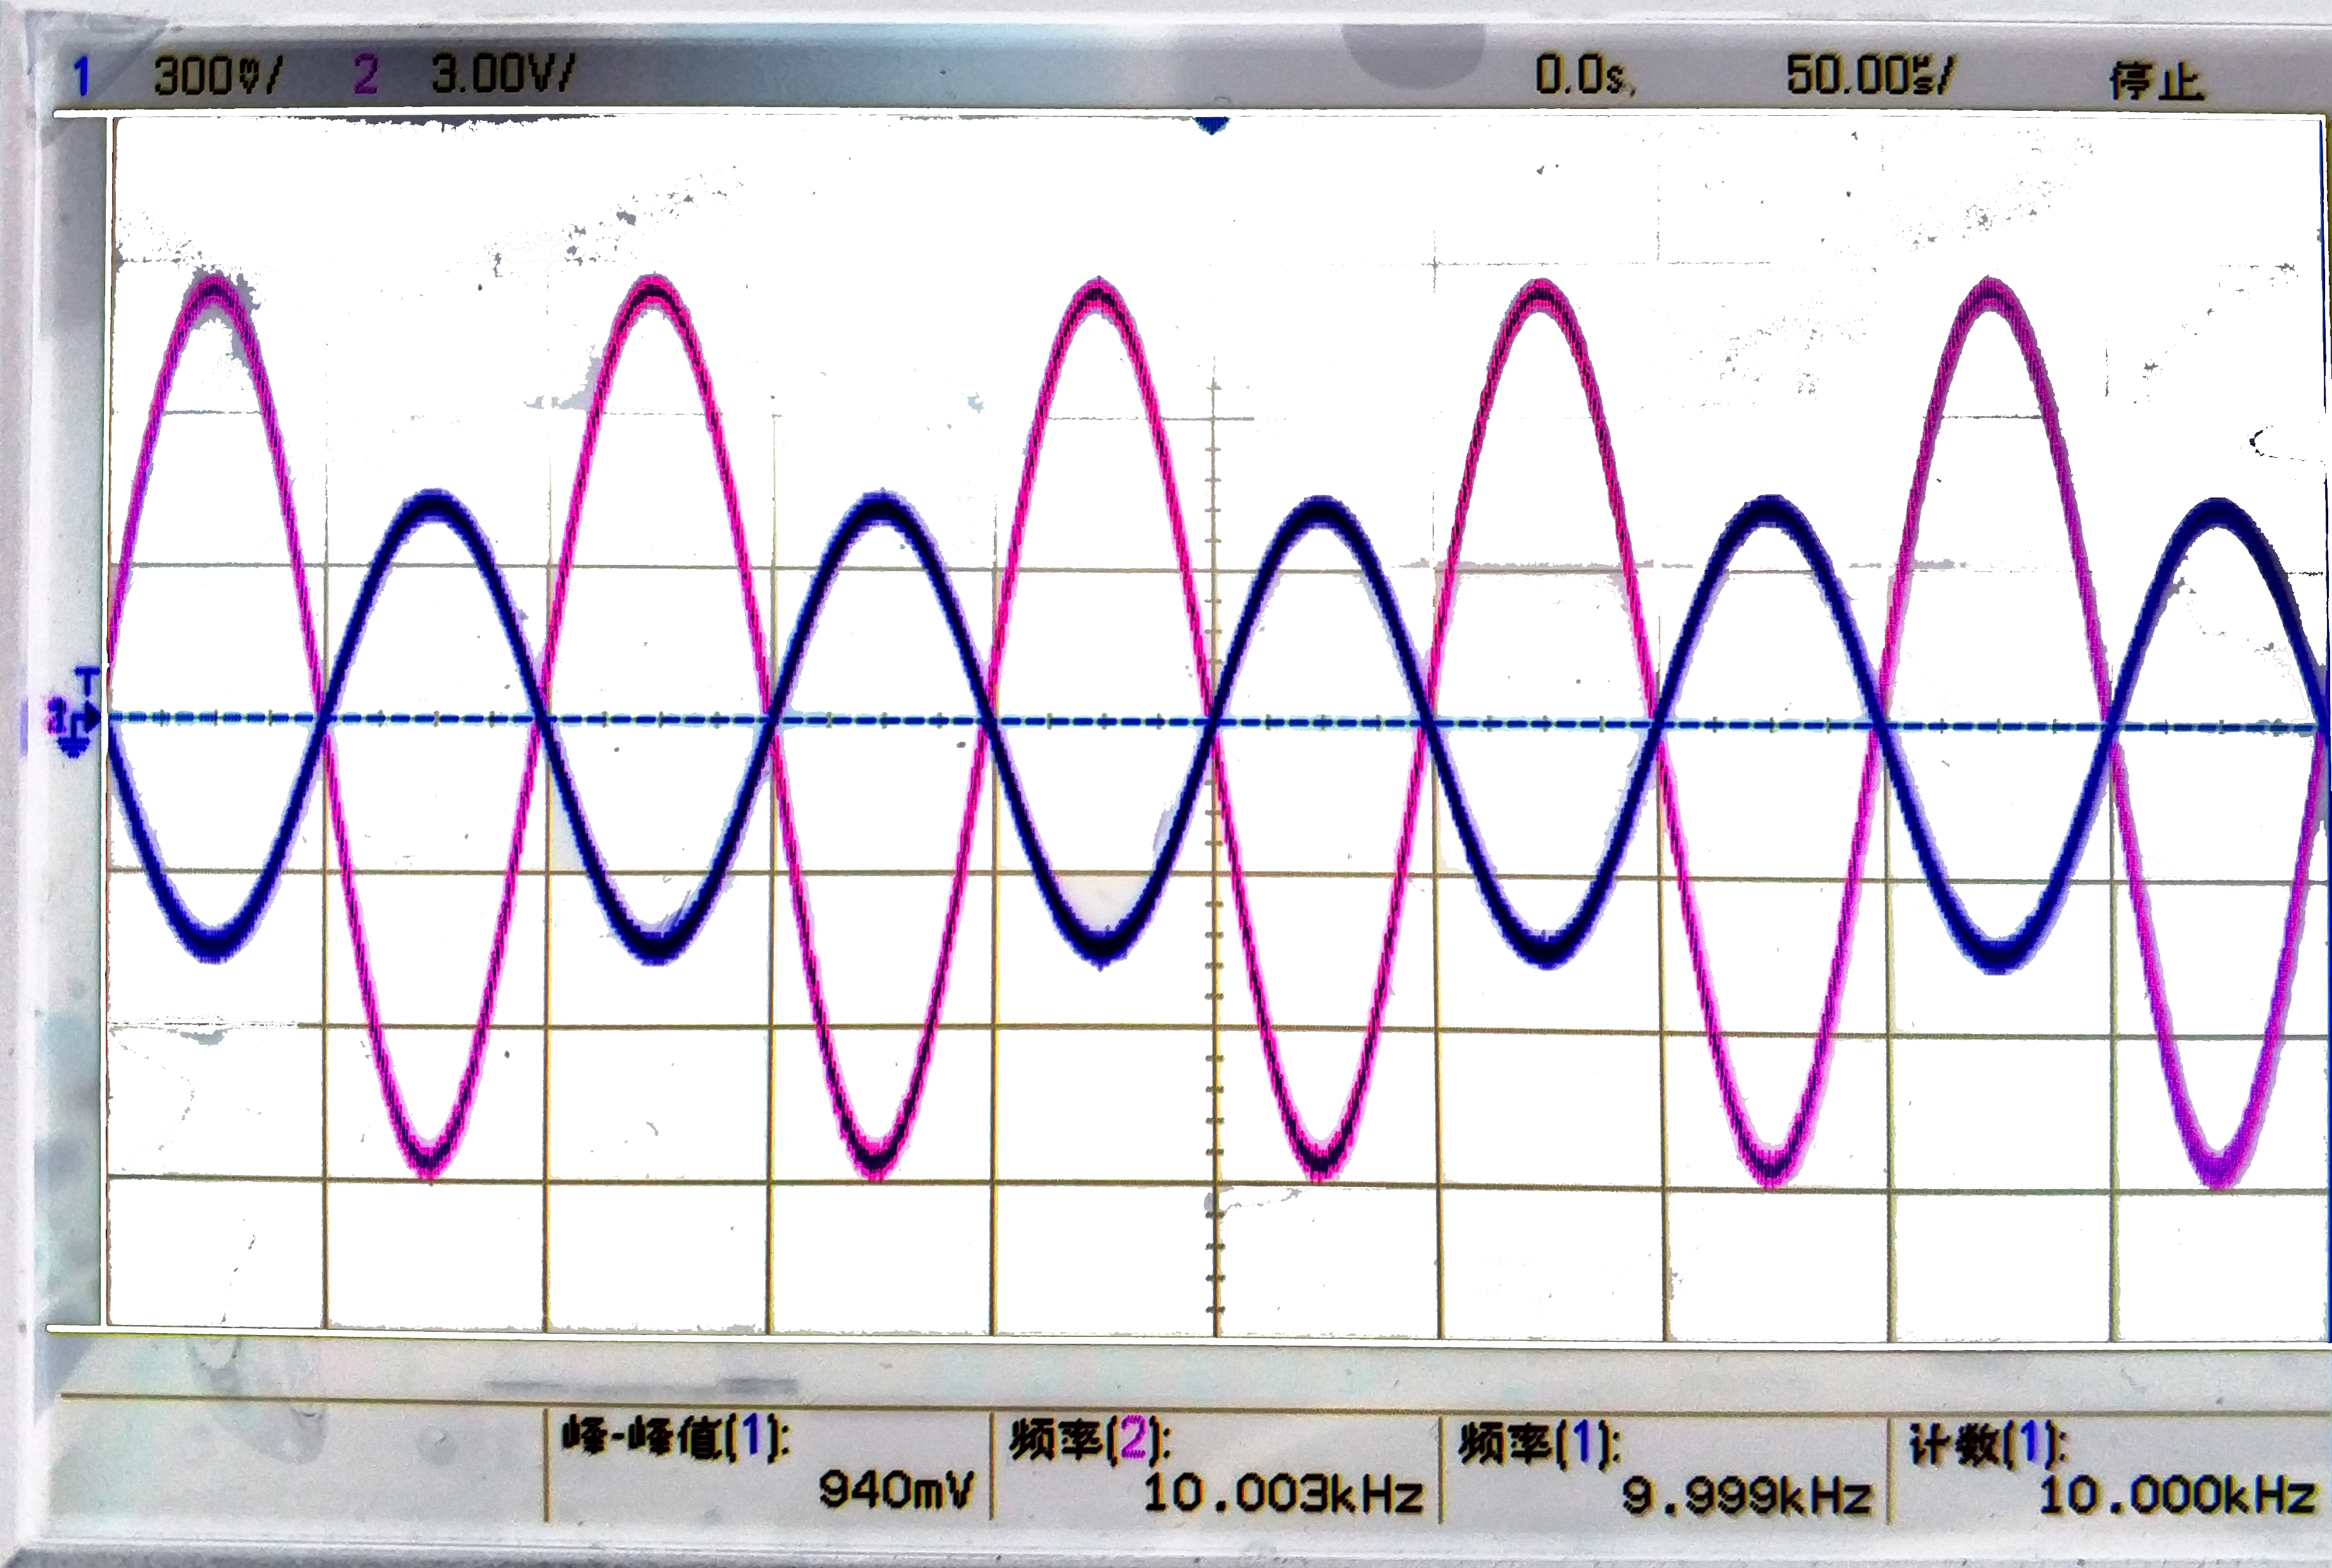
\includegraphics[width=12cm]{fig/waveform.jpg}\\
\caption{输入输出波形示意图}\label{wf}
\end{figure}

\textbf{理论值计算}:\\
根据教材$^{\cite{jiaocai}}$的式(5.3.7b):
\begin{equation}
r_{be} = r_{bb'} + (1+\beta)\frac{26mV}{I_{EQ}}\label{rbe}
\end{equation}
及例(5.3.2)中的:
\begin{equation}
I_{EQ} \approx \beta I_{BQ}=261.15\times4.505 =1176.48 \mu\text{A}
\end{equation}
结合实际情况,取$r_{bb'} = 800\Omega$,可得:
\begin{equation}
r_{be} = 800\Omega + (1+261.15)\cfrac{26\text{mV}}{1176.48 \mu\text{A}} = 6.59\text{k}\Omega
\end{equation}
再根据式(5.3.8)并进行适当修正,有(下文计算中略去负号):
\begin{equation}
A_v = \cfrac{v_o}{v_i} = -\cfrac{\beta(R_L||R_c)}{R_b||r_{be}}\label{Av}
\end{equation}
\begin{enumerate}
\item 空载\\
空载即$R_L = 0$,将各数据代入式(\ref{Av})即得理论放大倍数:
\begin{equation}
A_v = -\cfrac{261.15\times5.1\text{k}\Omega}{73.711\text{k}\Omega || 6.59\text{k}\Omega} \approx 220.17
\end{equation}
将理论值与实验测量值填入表(\ref{table2}):
\begin{table}[!h]
\centering
\caption{测量交流放大电路(空载)}
\label{table2}
\begin{tabular}{c|c|c|c}
\hline
\multicolumn{2}{c|}{测量值} & 由测量值计算 & 理论估算值 \\ \hline
$v_i(mV)$   & $v_o(mV)$  & $A_V$  & $A_V$ \\ \hline
3                 & 0.5988         & 199.6    & 220.17      \\ \hline
6                 & 1.1950         & 199.2    & 220.17      \\ \hline
9                 & 1.7745         & 197.2    & 220.17      \\ \hline
\end{tabular}
\end{table}

误差为:
\begin{eqnarray}
Error(v_i=3mV) &=& \frac{199.6-220.17}{220.17}\times 100\% = -9.30\%\\
Error(v_i=6mV) &=& \frac{199.2-220.17}{220.17}\times 100\% = -9.48\%\\
Error(v_i=9mV) &=& \frac{197.2-220.17}{220.17}\times 100\% = -10.39\%
\end{eqnarray}
\item 有载\\
有载即$R_L = 5.1\text{k}\Omega$和$R_L = 2.2\text{k}\Omega$,将各数据代入式(\ref{Av})即得理论放大倍数:
\begin{eqnarray}
A_v &=& -\cfrac{261.15\times(5.1\text{k}\Omega || 5.1\text{k}\Omega)}{73.711\text{k}\Omega || 6.59\text{k}\Omega} \approx 110.09\\
A_v &=& -\cfrac{261.15\times(5.1\text{k}\Omega || 2.2\text{k}\Omega)}{73.711\text{k}\Omega || 6.59\text{k}\Omega} \approx 66.35
\end{eqnarray}
\begin{table}[!h]
\centering
\caption{测量交流放大倍数(有载)}
\label{table4}
\begin{tabular}{c|c|c|c|c}
\hline
负载           & \multicolumn{2}{c|}{测量值}                 & 由测量值计算 & 理论估算值 \\ \hline
$R_L$        & $v_i(mV)$ & $v_o(mV)$ & $A_V$  & $A_V$ \\ \hline
5.1$k\Omega$ & 3.009 & 0.3055        & 101.5    & 110.09      \\ \hline
2.2$k\Omega$ & 3.009 & 0.1866        & 62.0      & 66.35     \\ \hline
\end{tabular}
\end{table}

误差为:
\begin{eqnarray}
Error(R_L = 5.1\text{k}\Omega) &=& \frac{101.5-110.09}{110.09}\times 100\% = -7.80\%\\
Error(R_L = 2.2\text{k}\Omega) &=& \frac{101.5-110.09}{110.09}\times 100\% = -6.56ff\%
\end{eqnarray}
\end{enumerate}
\item 空载幅频响应(通频带)\\
取中频为10kHz,$v_{o,rms} = 3.091 mV$得出$\frac{v_o}{\sqrt{2}} = 2.1857 mV$。测得对应的通频带为:\\下限$f_L$ = 860Hz,上限$f_H$ = 570kHz。
\item 输入输出电阻\\
\textbf{理论值计算:}\\
根据教材(5.3.9)和(5.3.10)两式,可以得出输入输出电阻的理论值:
\begin{eqnarray}
r_i &=& R_b || r_{be} = 73.711\text{k}\Omega || 6.59\text{k}\Omega = 6.05\text{k}\Omega\\
r_o &\approx& R_c = 5.1\text{k}\Omega
\end{eqnarray}
\begin{table}[!h]
\centering
\caption{测量输入输出电阻}
\label{table8}
\begin{tabular}{c|c|c|c|c|c|c|c}
\hline
\multicolumn{4}{c|}{测输入电阻$r_i$ $R_s = 5.1k\Omega$} & \multicolumn{4}{c}{测输出电阻$r_o$}                             \\ \hline
\multicolumn{2}{c|}{测量值}     & 测量计算值    & 理论估算值    & \multicolumn{2}{c|}{测量值}                    & 测量计算值 & 理论估算值 \\ \hline
$V_s(mV)$     & $V_i(mV)$    & $r_i$    & $r_i$    & $V_o, R_L\to\infty$ & $V_o, R_L=5.1k\Omega$ & $r-o$ & $r_o$ \\ \hline
36  &  18.828   & 5.6 k$\Omega$ & 6.05\text{k}$\Omega$ & 0.5988  & 0.3055  & 4.9k$\Omega$  & 5.1\text{k}$\Omega$ \\ \hline
\end{tabular}
\end{table}
则输入输出电阻的误差为:
\begin{eqnarray}
Error(r_i) &=& \cfrac{5.6\text{k}\Omega - 6.05\text{k}\Omega}{6.05\text{k}\Omega}\times 100\% = -7.44\%\\
Error(r_o) &=& \cfrac{4.9\text{k}\Omega - 5.1\text{k}\Omega}{5.1\text{k}\Omega}\times 100\% = -3.92\%
\end{eqnarray}
\item 空载谐波失真\\
空载谐波失真测量相关数据如下:
\begin{eqnarray*}
L_1 &=& -5.623 \text{ dB}\\
L_2 &=& -36.577 \text{ dB}\\
L_3 &=& -51.256 \text{ dB}
\end{eqnarray*}
\begin{eqnarray*}
d_{o2} &=& 10^{\cfrac{L_2-L_1}{20}}\times 100\% = 2.83\%\\
d_{o3} &=& 10^{\cfrac{L_3-L_1}{20}}\times 100\% = 0.52\%
\end{eqnarray*}
\end{enumerate}
\section{误差分析}
\iffalse
\begin{enumerate}
\item $r_{bb'}$的数值\\
式(\ref{rbe})中的$r_{be}$数值与掺杂浓度及制造工艺有关,而在本实验中并没有方法知道$r_{be}$的精确值。教材中例题的取值为200$\Omega$,此时误差约为20\%;而我在处理数据时使用的$r_{be}$为800$\Omega$,误差约为10\%。因此$r_{be}$的值不确定是误差的一个重要来源。
\item 测量误差\\
测量过程中发现,仪器的读数并不稳定,有时会出现随时间递增或递减的现象。这就给读数的准确性造成影响。尤其是当读数特别小,如$I_b$为$\mu$A量级时影响更为严重。
\end{enumerate}
\fi

\section{思考题}
\subsection{降低低频截止频率的方法。}
\subsection{减小非线性谐波失真的方法。}
%\subsection{实验体会。}

\bibliography{ref}
\end{document}